%{
%Formattting
\documentclass[12pt,a4paper]{article}
\usepackage[T1]{fontenc}
\usepackage[utf8]{inputenc}
\usepackage[left=0.75in, right=0.75in, bottom=1.1in]{geometry}
\usepackage[skip=7pt plus1pt, indent=0pt]{parskip}

\usepackage{fancyheadings}
\usepackage{setspace}
\usepackage{enumitem}
\usepackage{longtable}
\usepackage{array} % include this in your preamble

\usepackage{multicol}
\setlength\columnseprule{0.4pt}
%\setlength{\parindent}{0in}
\usepackage{listings}

\lstset
{ %Formatting for code in appendix
	basicstyle=\footnotesize,
	numbers=left,
	stepnumber=1,
	showstringspaces=false,
	tabsize=1,
	breaklines=true,
	breakatwhitespace=false
}

\usepackage{xargs} 
\usepackage[pdftex,dvipsnames]{xcolor}

%Mathematics
\usepackage{amsmath}
\usepackage{amsthm}
\usepackage{amssymb}
\usepackage{polynom}
\usepackage{mathtools}
\usepackage{float}
\usepackage{aliascnt}

\newaliascnt{eqfloat}{equation}
\newfloat{eqfloat}{h}{eqflts}
\floatname{eqfloat}{Equation}
\newcommand*{\ORGeqfloat}{}
\let\ORGeqfloat\eqfloat
\def\eqfloat{%
	\let\ORIGINALcaption\caption
	\def\caption{%
		\addtocounter{equation}{-1}%
		\ORIGINALcaption
	}%
	\ORGeqfloat
}
\usepackage{upgreek}

\usepackage{pict2e}

%Professor Latex Commands:
\newcommand{\tr}{\mathrm{tr}}
\newcommand{\ra}{\rightarrow}
\newcommand{\lan}{\langle}
\newcommand{\ran}{\rangle}
\newcommand{\norm}[1]{\left\lVert#1\right\rVert}
\newcommand{\inn}[1]{\lan#1\ran}
\newcommand{\ol}{\overline}
\newcommand{\F}{\mathbf{F}}
\newcommand{\M}{\mathcal{M}}
\newcommand{\res}{\text{Res}}
\newcommand{\ds}{\displaystyle}
\newcommand{\range}{\text{range}}

\makeatletter
\newcommand{\crossout}[1]{%
	\begingroup
	\settowidth{\dimen@}{#1}%
	\setlength{\unitlength}{0.05\dimen@}%
	\settoheight{\dimen@}{#1}%
	\count@=\dimen@
	\divide\count@ by \unitlength
	\begin{picture}(0,0)
		\put(0,0){\line(20,\count@){20}}
		\put(0,\count@){\line(20,-\count@){20}}
	\end{picture}%
	#1%
	\endgroup
}
\usepackage{tikz}
\newcommand\halmos{\rule{.36em}{2ex}}
\newcommand{\powerset}[1]{\mathcal{P}(#1)}
\def\contradict{\tikz[baseline, x=0.22em, y=0.22em, line width=0.032em]\draw (0,2.83)--(2.83,0) (0.71,3.54)--(3.54,0.71) (0,0.71)--(2.83,3.54) (0.71,0)--(3.54,2.83);}

%Citations
\usepackage[backend=biber,style=verbose-trad2]{biblatex} %works really really well, but no MLA format
%\addbibresource{references.bib}
\addbibresource{references.bib}
\nocite{*}

%Symbols and Other
\usepackage{upgreek}
\usepackage{graphicx}
\usepackage{animate}
\usepackage{caption}
\newcommand{\source}[1]{\caption*{Source: {#1}} }
\usepackage{hyperref}
\hypersetup{
	colorlinks,
	allcolors=black
	%citecolor=black,
	%filecolor=black,
	%linkcolor=black,
	%urlcolor=black
}
%onehalfspacing
\linespread{1}
%\doublespacing

\pagestyle{fancy}
\headheight 32pt

\usepackage{pdfpages}
%}

% Drafting 
%{
\usepackage[colorinlistoftodos,prependcaption, textsize=tiny]{todonotes}
\usepackage{lipsum}
\newcommandx{\unsure}[2][1=]{\todo[linecolor=red,backgroundcolor=red!25,bordercolor=red,#1]{#2}}
\newcommandx{\change}[2][1=]{\todo[linecolor=blue,backgroundcolor=blue!25,bordercolor=blue,#1]{#2}}
\newcommandx{\toadd}[2][1=]{\todo[linecolor=OliveGreen,backgroundcolor=OliveGreen!25,bordercolor=OliveGreen,#1]{#2}}
\newcommandx{\info}[2][1=]{\todo[linecolor=yellow,backgroundcolor=yellow!25,bordercolor=yellow,#1]{#2}}
\newcommandx{\improve}[2][1=]{\todo[linecolor=Plum,backgroundcolor=Plum!25,bordercolor=Plum,#1]{#2}}
\newcommandx{\hiddentodo}[2][1=]{\todo[disable,#1]{#2}}
%}
% ========================================= %
\newcommand{\doctitle}{Subsystem Design Specification}
\newcommand\team{University of Toronto Aerospace Team}	
\newcommand\subteam{Payload Electrical}  
\pagenumbering{gobble}
\begin{document}
    \title{\doctitle}
	\author{\team \\ \subteam}

	\maketitle
	
	\tableofcontents
    \thispagestyle{empty}
	
	\newpage
    \clearpage
    \pagenumbering{arabic}
    %So the heading doesn't show up on table of contents page
	%\lhead{\yourname\ \vspace{0.1cm} \\ \course}
	\lhead{\subteam}
    \chead{\textbf{\doctitle}}
    \rhead{July, 2025}

    \section{Subteam Overview}
    \subsection{System Introduction}
    The Payload Electrical team (PAY) is responsible for the electronics 
    necessary to control the payload. The payload for the FINCH mission
    is a pushbroom hyperspectral imager that uses the Teledyne FLIR Tau
    camera. The fact that the payload is such already implies a couple of 
    constraints: first, one spatial axis can be limited by the frame rate 
    of the system. Second, the system must be able to deal with a lot (a lot relative to the memory of the flash of the MCU used) in a short 
    amount of time which necessitates methods for rapid data transfer.

    In order to fulfill the mission requirements, not only do the electrical 
    interfaces need to be fast enough for data acquisition, the operations within
    the MCU must also be fast enough so as to not bottle neck the transfer of images
    to storage. The subsystem design specification exists to give an overview of the system:
    the electrical design, as well as methods to store the datacube. 
    
    \subsection{The Hardware We're Working With}
    \subsubsection{STM32H743IIT6}
    \begin{figure}[H]
        \centering
        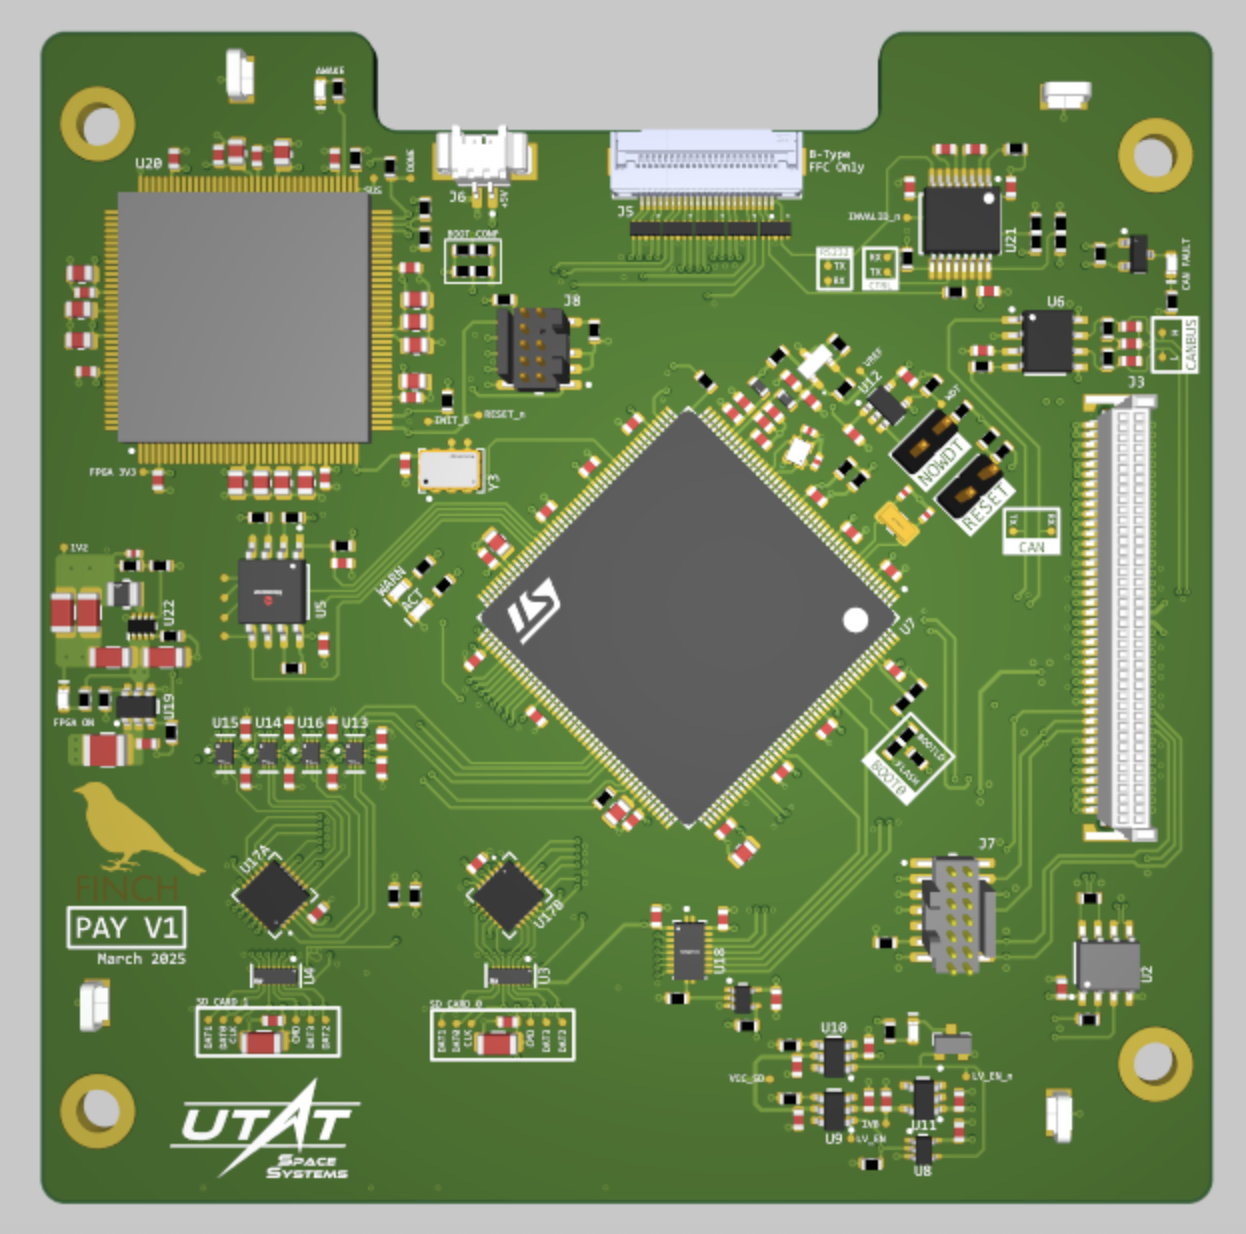
\includegraphics[width=0.5\linewidth]{../figures/PAY_SS.png}
        \caption{PAY v1.0}
    \end{figure}

    The Payload Electrical System utilizes an STM32H743IIT6 as the main 
    controller. The H7 has the following specs:

    \begin{table}[H]\centering
        \begin{tabular}{l | l}
            Core & Single Core \\
            & 32-bit ARM Cortex M7 \\ \hline
            Clocking & 480MHz Max \\ \hline
            On-chip Memory & 2 MBytes Flash \\
            & 1 MByte RAM \\ 
            & 512kB Largest DMA Chunk \\ \hline
            Peripherals & CAN \\
            & I2C \\
            & SPI \\
            & SDMMC \\
            & HDMI \\ \hline
            Package & LQFP-176\\ 
        \end{tabular}
        \caption{STM32H743IIT6 Relevant Electrical Specifications}
    \end{table}

    \subsubsection{FLIR TAU SWIR}
    \begin{figure}[H]
        \centering
            \begin{minipage}{0.49\linewidth}
            \centering
            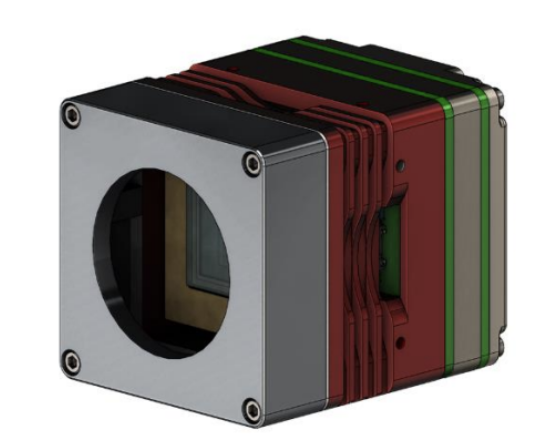
\includegraphics[width=1\textwidth]{../figures/tau_ss.png}
            \caption{\centering FLIR Tau SWIR}
            \label{fig:left_fig}
        \end{minipage}
        \begin{minipage}{0.4\linewidth}
            \centering
            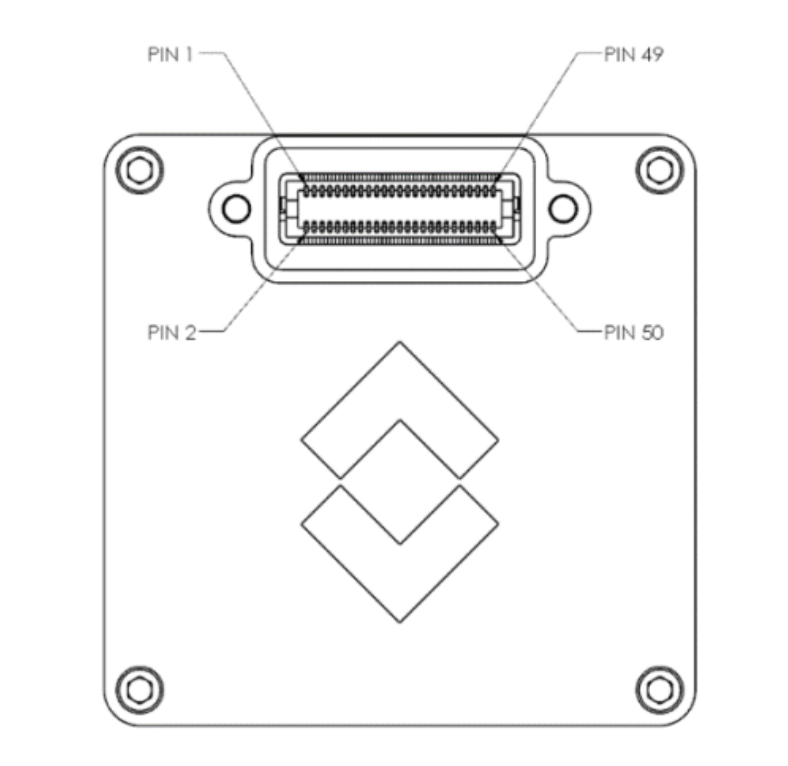
\includegraphics[width=1\textwidth]{../figures/tau_conn_ss.png}
            \caption{\centering FLIR Tau Connector}
            \label{fig:right_fig}
        \end{minipage}
    \end{figure}

    The camera used is the FLIR Tau SWIR. A few important notes about the use of 
    this camera: (1) A 256x320 subset of the detector is used rather than
    the 512x640 full frame. (2) image readout can be done while the camera is exposing\footcite{TAU_ProdSpec}. 
    (3) Commands are sent to the camera via RS232. (4) DCMI is used to readout 
    the image with a pixel clock of 5.7048MHz. (5) The 14-bit pixels are 
    stored in 2 bytes. (6) The team still needs to measure the QE of this camera. 

    For the 256x320 subset, the readout time is then given by 
    \begin{equation}
        \frac{256 \times 320}{f_{CLKPIX}} \approx 14.36\text{ms}
    \end{equation}

    Given this readout time, the max frame rate is then 
    \begin{equation}
        1 \text{ frame} / 14.36\text{ms} \approx 69.63 \text{fps}
    \end{equation}
    Of course, the actual frame rate will be less considering also the 
    time for commanding. 60fps should be a safe baseline for now. The docs claim a much faster frame rate of 120fps but we are assuming that 
    a buffer within a camera is what makes that possible. Assuming the buffer, 
    there must be a max number of frames that can be taken at 120fps and so this 
    will not be suitable for the FINCH mission since imaging would last to the 
    order of 30s. 

    \begin{table}[H]\centering
        \begin{tabular}{l | l}
            Resolution & 512x640 pixels \\
            & 14-bit analog resolution \\ \hline
            Commanding Interface & RS232 \\ \hline
            Data Interface & 14-bit DCMI\\
            & 5.7048MHz Pixel Clock\\
        \end{tabular}
        \caption{FLIR Tau SWIR Electrical Summary}
    \end{table}

    \subsubsection{SD Cards}
    The data is to be stored on SD cards onboard PAY. PAY has two SD cards that 
    it can access using a MUX. Hardware is implemented so that the logic level 
    can go down to 1.8V to enable greater than 25 MBytes/s transfer speed to the 
    SD card (UHS mode). More details on the SD cards are provided in 
    Section \ref{sec:Det_Sys_Arc}. 

    \subsubsection{Spartan 6 FPGA}
    Yes, there is an FPGA onboard. Initially, the FPGA was on the board for compression 
    which recently became a "Should" requirement. 



    \section{Applicable Documents and Standards}\label{sec:methods}
    \subsection{General Documents}
    \begin{itemize}
        \item PAY Datasheet
        \item Master Connection Sheet
        \item \cite{TAU_ProdSpec}
    \end{itemize}
    \subsection{Specifications, Standards, and Handbooks}
    \begin{itemize}
        \item Spacecraft Grounding: NASA-HDBK-4001
    \end{itemize}
   
    \newpage
    \section{Subsystem Requirements}\label{sec:requirements}

    \subsection{Electrical System Requirements}
    From the FINCH-Spacecraft-ElectricalSystem, requirements for the existence of OBC and PAY are derived. Seen in Table \ref{tab:elec_sys_req} are also other higher-lever requirements of the system including the common bus to connect OBC, PAY, and the board for the Electrical Power System (EPS).
    \begin{table}[H]
        \centering
        \begin{tabular}{|>{\centering\arraybackslash}m{3cm} 
                    |>{\raggedright\arraybackslash}m{7cm} 
                    |>{\centering\arraybackslash}m{3cm} 
                    |>{\centering\arraybackslash}m{2.5cm}|}\hline
            \textbf{Req. ID} & \centering \textbf{Description} & \textbf{Parent Req.} & \textbf{Verification Method}\\\hline
             FINCH-Spacecraft-ElectricalSystem&  The electrical system shall provide the necessary electrical functionality for the mission to function. &  FINCH-Mission-Objective& Demonstration\\\hline
 FINCH-OBC-ControlAndOps& The OBC shall control the modes of operation of the satellite. & FINCH-Spacecraft-ElectricalSystem&Demonstration\\\hline
 FINCH-Payload Controller-PayloadOps& The Payload Controller shall support necessary operations for executing the mission of the payload& FINCH-Spacecraft-ElectricalSystem&Demonstration\\\hline
             FINCH-Spacecraft-CommonBus&  The spacecraft shall utilize a common bus which includes the lines for power and communication between OBC, EPS, and PAY. &  FINCH-Spacecraft-ElectricalSystem& Test\\\hline
             FINCH-Spacecraft-CANBus&  The spacecraft shall use CAN Bus for communication between nodes on the electrical system.&  FINCH-Spacecraft-CommonBus& Test\\\hline
             FINCH-Spacecraft-Electrical Grounding&  The grounding system for the spacecraft shall include a separate chassis and signal ground.&  FINCH-Spacecraft-ElectricalSystem& Analysis\\\hline
             FINCH-Spacecraft-Electrical Soldering Standard&  Electrical components shall be soldered in accordance to IPC Type 3 or equivalent&  FINCH-Spacecraft-ElectricalSystem& Inspection\\\hline
        \end{tabular}
        \caption{Electrical System Requirements}\label{tab:elec_sys_req}
    \end{table}
    
    \subsection{PAY Requirements}
Figure \ref{fig:PAY_req_tree} and Table \ref{tab:pay_reqs}
summarize the requirements for the Payload Controller system. 

Notable is the compression requirement which has only become a "should" recently after PAY was designed. The reason why the requirement suddenly became a "should" comes from a spec from optics saying that the whole sensor will not be used. Initial requirement for compression assumed the whole sensor would be used. 
    \begin{figure}[H]
        \centering
        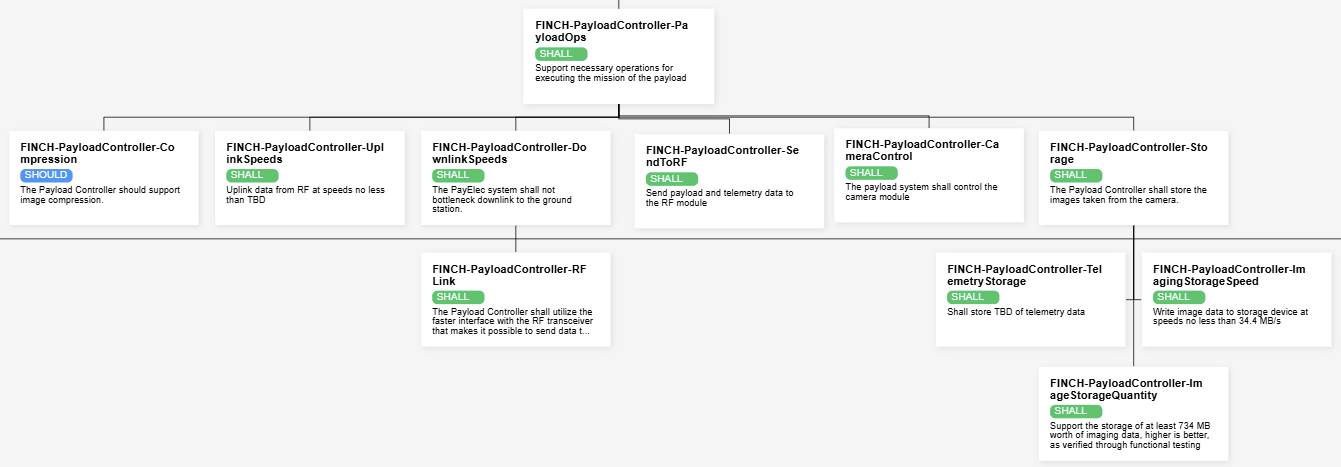
\includegraphics[width=1\linewidth]{../figures/PAY_req_tree.png}
        \caption{PAY Requirement Tree}
        \label{fig:PAY_req_tree}
    \end{figure}

    \begin{table}[H]
        \centering
        \begin{tabular}{|>{\centering\arraybackslash}m{3cm} 
                    |>{\raggedright\arraybackslash}m{7cm} 
                    |>{\centering\arraybackslash}m{3cm} 
                    |>{\centering\arraybackslash}m{2.5cm}|}\hline
            \textbf{Req. ID} & \centering \textbf{Description} & \textbf{Parent Req.} & \textbf{Verification Method}\\\hline
 FINCH-PayloadController-CameraControl& The Payload Controller shall control the camera module& FINCH-PayloadController-PayloadOps&Test, Analysis\\\hline
 FINCH-PayloadController-Storage& The Payload Controller shall store the images taken from the camera.& FINCH-PayloadController-Storage&Test\\\hline
 FINCH-PayloadController-ImagingStorageSpeed& The Payload Controller shall write image data to storage device at speeds no less than 34.4 MB/s& FINCH-PayloadController-Storage&Test\\\hline
 FINCH-PayloadController-ImageStorageQuantity& The Payload Controller shall support the storage of at least 734 MB worth of imaging data, higher is better, as verified through functional testing& FINCH-PayloadController-Storage&Test\\\hline
 FINCH-PayloadController-TelemetryStorage& The Payload Controller shall be capable of storing telemetry data.& FINCH-PayloadController-Storage&Test\\\hline
 FINCH-PayloadController-DownlinkSpeeds& The Payload Controller system shall not bottleneck downlink to the ground station. & FINCH-PayloadController-PayloadOps&Test\\\hline
 FINCH-PayloadController-RFLink& The Payload Controller shall utilize the faster interface with the RF transceiver that makes it possible to send data to the transceiver such that it does not bottleneck communication.& FINCH-PayloadController-DownlinkSpeeds&Test\\\hline
 FINCH-PayloadController-UplinkSpeeds& The Payload Controller system shall be capable of receiving data from the RF module directly. & FINCH-PayloadController-PayloadOps&Test\\\hline
 FINCH-PayloadController-SendToRF& The Payload Controller shall be capable of directly sending payload and telemetry data to the RF module.& FINCH-PayloadController-PayloadOps&Test\\\hline
 FINCH-PayloadController-Compression& The Payload Controller should support image compression.& FINCH-PayloadController-PayloadOps&Test\\\hline
        \end{tabular}
        \caption{Electrical System Requirements}\label{tab:pay_reqs}
    \end{table}

   
    
    \section{Verification and Validation Plan}\label{sec:verifcation_validation}
    Electrical requirements will be verified via tests and demonstrations. The verification and validation plan will follow the following timeline:
    


    \section{High Level System Architecture}
    \subsection{Grounding Scheme}
    The initial grounding scheme before the payload redesign was a Star grounding 
    scheme. This was easy since the boards were just stacked together and then 
    cables simply emanated from that stack. For the new mechanical layout, though, 
    the EPS board will be separate from the rest of the boards. 

    \section{Detailed System Architecture}\label{sec:Det_Sys_Arc}

    \section{Possible Risks}

    \section{Development Schedule and Status}

    \section{Open Issues and Future Work}

    \printbibliography
    
            
    \newpage
    \pagenumbering{roman}


    %\section{Uncertainty Calculations}




\end{document}

        \begin{figure}[h]
            \centering
             \begin{minipage}{0.49\linewidth}
                \centering
                \includegraphics[width=1\textwidth]{left figure}
                \caption{\centering left caption}
                \label{fig:left_fig}
            \end{minipage}
            \begin{minipage}{0.49\linewidth}
                \centering
                \includegraphics[width=1\textwidth]{right figure}
                \caption{\centering right caption}
                \label{fig:right_fig}
            \end{minipage}
        \end{figure}

          % \begin{equation}
    %     \begin{split}
    %         Z_{in} &= \left( \frac{1}{r_b} + \frac{1}{Z_{base}} \right)^{-1} \\
    %         &= \left( \frac{1}{r_b} + \frac{i_b}{i_e (r'_e + R_{sw}))} \right)^{-1} 
    %     \end{split}
    % \end{equation}

    % $i_e = i_c + i_b = i_b(\beta + 1)\approx \beta i_b = i_c$ for $\beta \gg 1$. This approximation often holds as $\beta$ is usually large. Making this approximation,

    % \begin{equation}
    %     \begin{split}
    %         Z_{in} &= \left( \frac{1}{r_b} + \frac{1}{\beta (r'_e + R_{sw})} \right)^{-1} \\
    %          &= \frac{\beta r_b(r'_e + R_{sw})}{\beta (r'_e + R_{sw}) + r_b}
    %     \end{split}
    % \end{equation}
    
    % \begin{equation}
    %     A_V = \frac{v_{out}}{v_{in}} = \frac{-r_c i_c}{i_e }
    % \end{equation}

    % The gain of 

    % From Equation \eqref{eqn:r'_e}, $i_c$ must be determined to solve for $r'_e$. From Equation \eqref{eqn:transistor_eqn}, $i_c$ can be found knowing $i_b$. By Kirchoff's voltage law on the loop containing $r_b$, $r'_e$, and $R_{sw}$ on the AC equivalent circuit, 
    % \begin{equation}
    %     r_b i_b = (r'_e + R_{sw})i_e 
    % \end{equation}
    % $i_e = i_c + i_b = i_b(\beta + 1)\approx \beta i_b = i_c$ for $\beta \gg 1$. This approximation often holds as $\beta$ is usually large. Making this approximation,
    % \begin{equation}
    %     \begin{split}
    %         i_c &= \frac{r_b i_b}{(r'_e + R_{sw})}\\
    %          %&= \frac{r_b}{\beta{(r'_e + R_{sw})}}
    %          \label{eqn:collector_current}
    %     \end{split}
    % \end{equation}
    % Using this in equation \eqref{eqn:r'_e},
    % \begin{equation}
    %     r'_e = \frac{R_{sw}}{\frac{r_b}{\beta \kappa_T} }
    % \end{equation}
